\documentclass[1p]{elsarticle_modified}
%\bibliographystyle{elsarticle-num}

%\usepackage[colorlinks]{hyperref}
%\usepackage{abbrmath_seonhwa} %\Abb, \Ascr, \Acal ,\Abf, \Afrak
\usepackage{amsfonts}
\usepackage{amssymb}
\usepackage{amsmath}
\usepackage{amsthm}
\usepackage{scalefnt}
\usepackage{amsbsy}
\usepackage{kotex}
\usepackage{caption}
\usepackage{subfig}
\usepackage{color}
\usepackage{graphicx}
\usepackage{xcolor} %% white, black, red, green, blue, cyan, magenta, yellow
\usepackage{float}
\usepackage{setspace}
\usepackage{hyperref}

\usepackage{tikz}
\usetikzlibrary{arrows}

\usepackage{multirow}
\usepackage{array} % fixed length table
\usepackage{hhline}

%%%%%%%%%%%%%%%%%%%%%
\makeatletter
\renewcommand*\env@matrix[1][\arraystretch]{%
	\edef\arraystretch{#1}%
	\hskip -\arraycolsep
	\let\@ifnextchar\new@ifnextchar
	\array{*\c@MaxMatrixCols c}}
\makeatother %https://tex.stackexchange.com/questions/14071/how-can-i-increase-the-line-spacing-in-a-matrix
%%%%%%%%%%%%%%%

\usepackage[normalem]{ulem}

\newcommand{\msout}[1]{\ifmmode\text{\sout{\ensuremath{#1}}}\else\sout{#1}\fi}
%SOURCE: \msout is \stkout macro in https://tex.stackexchange.com/questions/20609/strikeout-in-math-mode

\newcommand{\cancel}[1]{
	\ifmmode
	{\color{red}\msout{#1}}
	\else
	{\color{red}\sout{#1}}
	\fi
}

\newcommand{\add}[1]{
	{\color{blue}\uwave{#1}}
}

\newcommand{\replace}[2]{
	\ifmmode
	{\color{red}\msout{#1}}{\color{blue}\uwave{#2}}
	\else
	{\color{red}\sout{#1}}{\color{blue}\uwave{#2}}
	\fi
}

\newcommand{\Sol}{\mathcal{S}} %segment
\newcommand{\D}{D} %diagram
\newcommand{\A}{\mathcal{A}} %arc


%%%%%%%%%%%%%%%%%%%%%%%%%%%%%5 test

\def\sl{\operatorname{\textup{SL}}(2,\Cbb)}
\def\psl{\operatorname{\textup{PSL}}(2,\Cbb)}
\def\quan{\mkern 1mu \triangleright \mkern 1mu}

\theoremstyle{definition}
\newtheorem{thm}{Theorem}[section]
\newtheorem{prop}[thm]{Proposition}
\newtheorem{lem}[thm]{Lemma}
\newtheorem{ques}[thm]{Question}
\newtheorem{cor}[thm]{Corollary}
\newtheorem{defn}[thm]{Definition}
\newtheorem{exam}[thm]{Example}
\newtheorem{rmk}[thm]{Remark}
\newtheorem{alg}[thm]{Algorithm}

\newcommand{\I}{\sqrt{-1}}
\begin{document}

%\begin{frontmatter}
%
%\title{Boundary parabolic representations of knots up to 8 crossings}
%
%%% Group authors per affiliation:
%\author{Yunhi Cho} 
%\address{Department of Mathematics, University of Seoul, Seoul, Korea}
%\ead{yhcho@uos.ac.kr}
%
%
%\author{Seonhwa Kim} %\fnref{s_kim}}
%\address{Center for Geometry and Physics, Institute for Basic Science, Pohang, 37673, Korea}
%\ead{ryeona17@ibs.re.kr}
%
%\author{Hyuk Kim}
%\address{Department of Mathematical Sciences, Seoul National University, Seoul 08826, Korea}
%\ead{hyukkim@snu.ac.kr}
%
%\author{Seokbeom Yoon}
%\address{Department of Mathematical Sciences, Seoul National University, Seoul, 08826,  Korea}
%\ead{sbyoon15@snu.ac.kr}
%
%\begin{abstract}
%We find all boundary parabolic representation of knots up to 8 crossings.
%
%\end{abstract}
%\begin{keyword}
%    \MSC[2010] 57M25 
%\end{keyword}
%
%\end{frontmatter}

%\linenumbers
%\tableofcontents
%
\newcommand\colored[1]{\textcolor{white}{\rule[-0.35ex]{0.8em}{1.4ex}}\kern-0.8em\color{red} #1}%
%\newcommand\colored[1]{\textcolor{white}{ #1}\kern-2.17ex	\textcolor{white}{ #1}\kern-1.81ex	\textcolor{white}{ #1}\kern-2.15ex\color{red}#1	}

{\Large $\underline{10_{50}~(K10a_{82})}$}

\setlength{\tabcolsep}{10pt}
\renewcommand{\arraystretch}{1.6}
\vspace{1cm}\begin{tabular}{m{100pt}>{\centering\arraybackslash}m{274pt}}
\multirow{5}{120pt}{
	\centering
	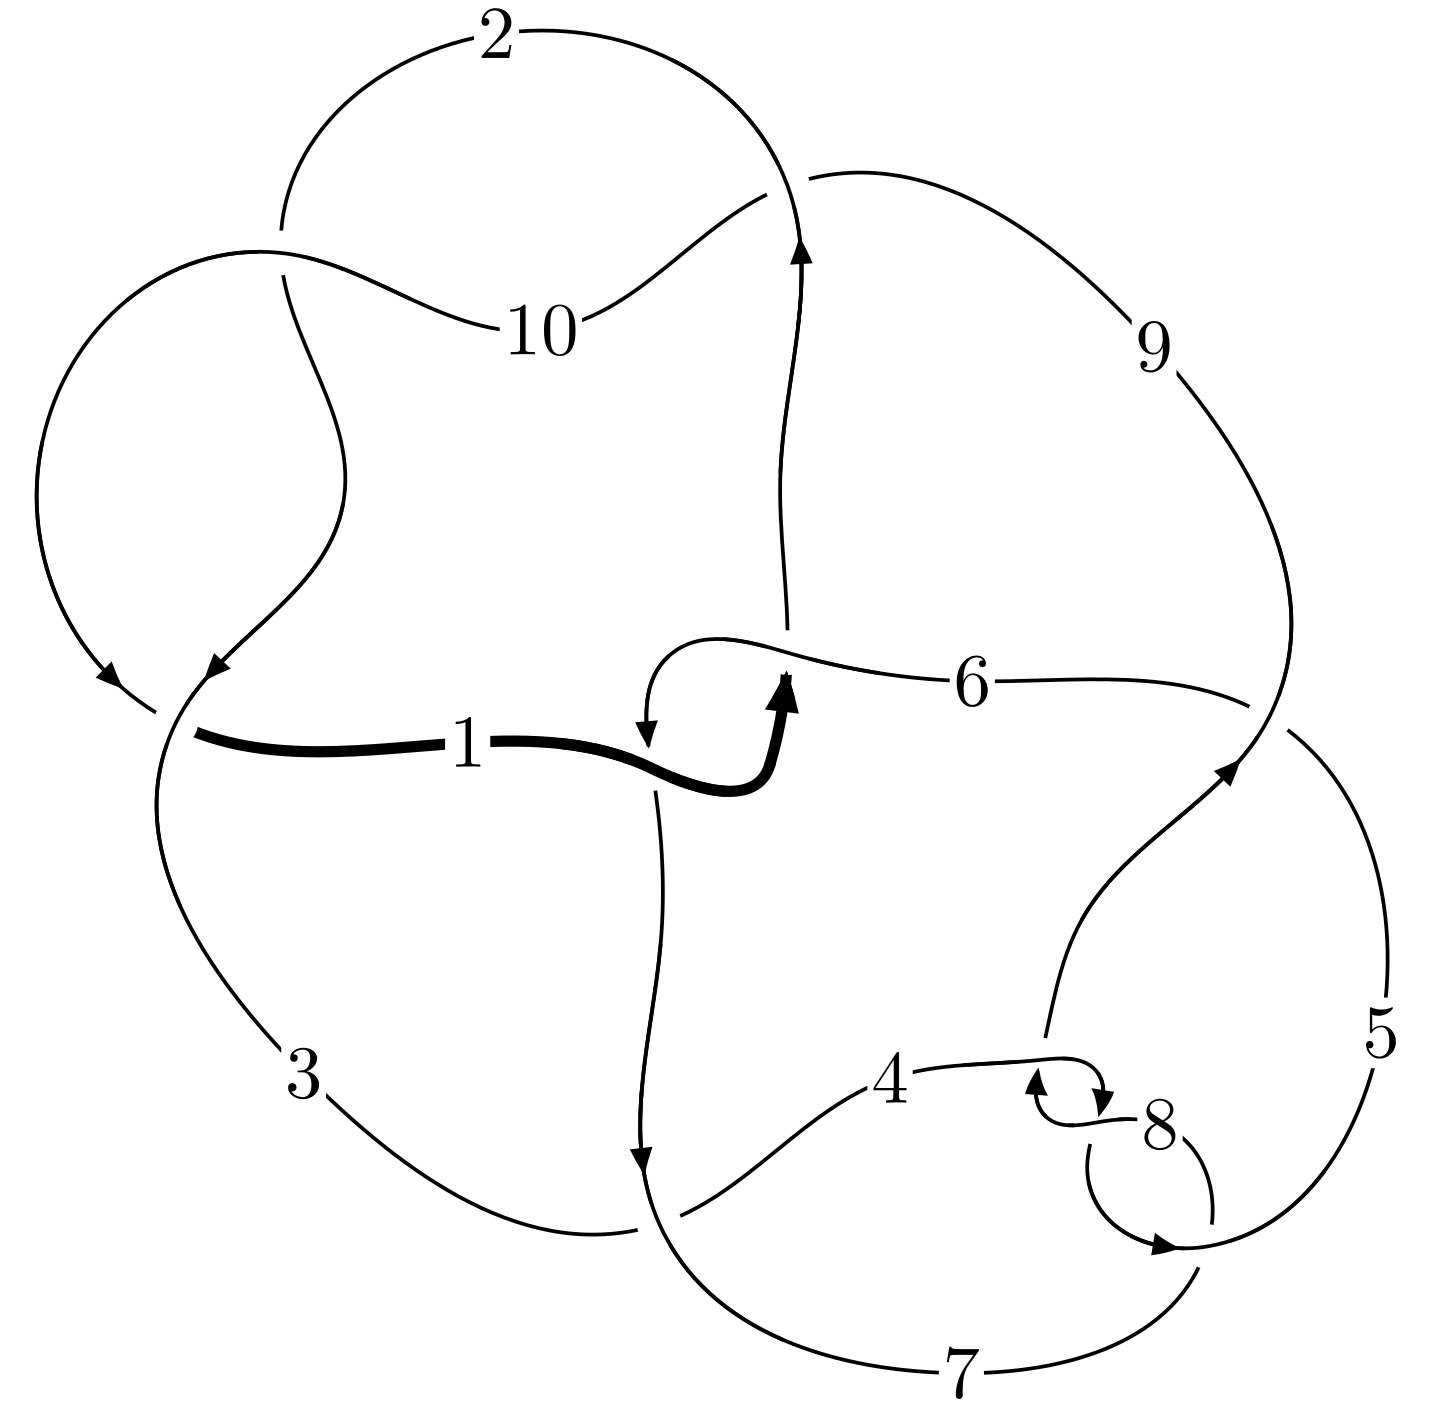
\includegraphics[width=112pt]{../../../GIT/diagram.site/Diagrams/png/134_10_50.png}\\
\ \ \ A knot diagram\footnotemark}&
\allowdisplaybreaks
\textbf{Linearized knot diagam} \\
\cline{2-2}
 &
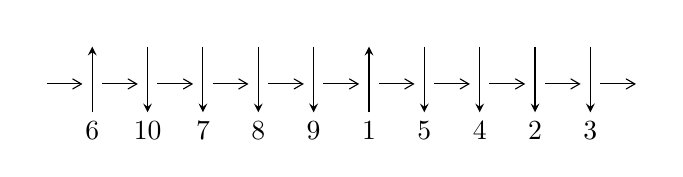
\begin{tikzpicture}[x=20pt, y=17pt]
	% nodes
	\node (C0) at (0, 0) {};
	\node (C1) at (1, 0) {};
	\node (C1U) at (1, +1) {};
	\node (C1D) at (1, -1) {6};

	\node (C2) at (2, 0) {};
	\node (C2U) at (2, +1) {};
	\node (C2D) at (2, -1) {10};

	\node (C3) at (3, 0) {};
	\node (C3U) at (3, +1) {};
	\node (C3D) at (3, -1) {7};

	\node (C4) at (4, 0) {};
	\node (C4U) at (4, +1) {};
	\node (C4D) at (4, -1) {8};

	\node (C5) at (5, 0) {};
	\node (C5U) at (5, +1) {};
	\node (C5D) at (5, -1) {9};

	\node (C6) at (6, 0) {};
	\node (C6U) at (6, +1) {};
	\node (C6D) at (6, -1) {1};

	\node (C7) at (7, 0) {};
	\node (C7U) at (7, +1) {};
	\node (C7D) at (7, -1) {5};

	\node (C8) at (8, 0) {};
	\node (C8U) at (8, +1) {};
	\node (C8D) at (8, -1) {4};

	\node (C9) at (9, 0) {};
	\node (C9U) at (9, +1) {};
	\node (C9D) at (9, -1) {2};

	\node (C10) at (10, 0) {};
	\node (C10U) at (10, +1) {};
	\node (C10D) at (10, -1) {3};
	\node (C11) at (11, 0) {};

	% arrows
	\draw[->,>={angle 60}]
	(C0) edge (C1) (C1) edge (C2) (C2) edge (C3) (C3) edge (C4) (C4) edge (C5) (C5) edge (C6) (C6) edge (C7) (C7) edge (C8) (C8) edge (C9) (C9) edge (C10) (C10) edge (C11) ;	\draw[->,>=stealth]
	(C1D) edge (C1U) (C2U) edge (C2D) (C3U) edge (C3D) (C4U) edge (C4D) (C5U) edge (C5D) (C6D) edge (C6U) (C7U) edge (C7D) (C8U) edge (C8D) (C9U) edge (C9D) (C10U) edge (C10D) ;
	\end{tikzpicture} \\
\hhline{~~} \\& 
\textbf{Solving Sequence} \\ \cline{2-2} 
 &
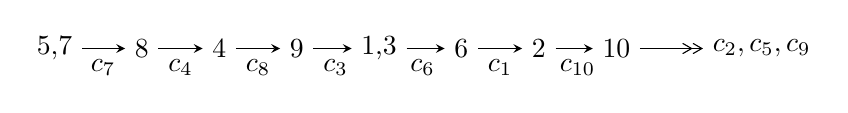
\begin{tikzpicture}[x=28pt, y=7pt]
	% node
	\node (A0) at (-1/8, 0) {5,7};
	\node (A1) at (1, 0) {8};
	\node (A2) at (2, 0) {4};
	\node (A3) at (3, 0) {9};
	\node (A4) at (65/16, 0) {1,3};
	\node (A5) at (41/8, 0) {6};
	\node (A6) at (49/8, 0) {2};
	\node (A7) at (57/8, 0) {10};
	\node (C1) at (1/2, -1) {$c_{7}$};
	\node (C2) at (3/2, -1) {$c_{4}$};
	\node (C3) at (5/2, -1) {$c_{8}$};
	\node (C4) at (7/2, -1) {$c_{3}$};
	\node (C5) at (37/8, -1) {$c_{6}$};
	\node (C6) at (45/8, -1) {$c_{1}$};
	\node (C7) at (53/8, -1) {$c_{10}$};
	\node (A8) at (9, 0) {$c_{2},c_{5},c_{9}$};

	% edge
	\draw[->,>=stealth]	
	(A0) edge (A1) (A1) edge (A2) (A2) edge (A3) (A3) edge (A4) (A4) edge (A5) (A5) edge (A6) (A6) edge (A7) ;
	\draw[->>,>={angle 60}]	
	(A7) edge (A8);
\end{tikzpicture} \\ 

\end{tabular} \\

\footnotetext{
The image of knot diagram is generated by the software ``\textbf{Draw programme}" developed by Andrew Bartholomew(\url{http://www.layer8.co.uk/maths/draw/index.htm\#Running-draw}), where we modified some parts for our purpose(\url{https://github.com/CATsTAILs/LinksPainter}).
}\phantom \\ \newline 
\centering \textbf{Ideals for irreducible components\footnotemark of $X_{\text{par}}$} 
 
\begin{align*}
I^u_{1}&=\langle 
u^{28}-2 u^{27}+\cdots+b+1,\;2 u^{28}-2 u^{27}+\cdots+a+2,\;u^{29}-2 u^{28}+\cdots+u-1\rangle \\
I^u_{2}&=\langle 
b,\;u^2+a+1,\;u^3+u^2+2 u+1\rangle \\
\\
\end{align*}
\raggedright * 2 irreducible components of $\dim_{\mathbb{C}}=0$, with total 32 representations.\\
\footnotetext{All coefficients of polynomials are rational numbers. But the coefficients are sometimes approximated in decimal forms when there is not enough margin.}
\newpage
\renewcommand{\arraystretch}{1}
\centering \section*{I. $I^u_{1}= \langle u^{28}-2 u^{27}+\cdots+b+1,\;2 u^{28}-2 u^{27}+\cdots+a+2,\;u^{29}-2 u^{28}+\cdots+u-1 \rangle$}
\flushleft \textbf{(i) Arc colorings}\\
\begin{tabular}{m{7pt} m{180pt} m{7pt} m{180pt} }
\flushright $a_{5}=$&$\begin{pmatrix}0\\u\end{pmatrix}$ \\
\flushright $a_{7}=$&$\begin{pmatrix}1\\0\end{pmatrix}$ \\
\flushright $a_{8}=$&$\begin{pmatrix}1\\u^2\end{pmatrix}$ \\
\flushright $a_{4}=$&$\begin{pmatrix}u\\u^3+u\end{pmatrix}$ \\
\flushright $a_{9}=$&$\begin{pmatrix}u^2+1\\u^4+2 u^2\end{pmatrix}$ \\
\flushright $a_{1}=$&$\begin{pmatrix}-2 u^{28}+2 u^{27}+\cdots-6 u-2\\- u^{28}+2 u^{27}+\cdots+u-1\end{pmatrix}$ \\
\flushright $a_{3}=$&$\begin{pmatrix}u^3+2 u\\u^3+u\end{pmatrix}$ \\
\flushright $a_{6}=$&$\begin{pmatrix}- u^5-2 u^3- u\\- u^7-3 u^5-2 u^3+u\end{pmatrix}$ \\
\flushright $a_{2}=$&$\begin{pmatrix}- u^{16}-7 u^{14}+\cdots-6 u-1\\u^{28}-2 u^{27}+\cdots- u^2+1\end{pmatrix}$ \\
\flushright $a_{10}=$&$\begin{pmatrix}- u^{28}+u^{27}+\cdots-5 u-1\\u^{17}+7 u^{15}+\cdots+6 u^2+u\end{pmatrix}$\\&\end{tabular}
\flushleft \textbf{(ii) Obstruction class $= -1$}\\~\\
\flushleft \textbf{(iii) Cusp Shapes $= u^{28}-2 u^{27}+17 u^{26}-28 u^{25}+121 u^{24}-169 u^{23}+476 u^{22}-572 u^{21}+1124 u^{20}-1170 u^{19}+1569 u^{18}-1418 u^{17}+1069 u^{16}-834 u^{15}-98 u^{14}+112 u^{13}-636 u^{12}+544 u^{11}-270 u^{10}+426 u^9-12 u^8+183 u^7-90 u^6-34 u^5-38 u^4-76 u^3+29 u^2+2 u-3$}\\~\\
\newpage\renewcommand{\arraystretch}{1}
\flushleft \textbf{(iv) u-Polynomials at the component}\newline \\
\begin{tabular}{m{50pt}|m{274pt}}
Crossings & \hspace{64pt}u-Polynomials at each crossing \\
\hline $$\begin{aligned}c_{1},c_{6}\end{aligned}$$&$\begin{aligned}
&u^{29}+u^{28}+\cdots-4 u-8
\end{aligned}$\\
\hline $$\begin{aligned}c_{2},c_{9},c_{10}\end{aligned}$$&$\begin{aligned}
&u^{29}-4 u^{28}+\cdots+2 u-1
\end{aligned}$\\
\hline $$\begin{aligned}c_{3},c_{5}\end{aligned}$$&$\begin{aligned}
&u^{29}+2 u^{28}+\cdots-15 u-9
\end{aligned}$\\
\hline $$\begin{aligned}c_{4},c_{7},c_{8}\end{aligned}$$&$\begin{aligned}
&u^{29}-2 u^{28}+\cdots+u-1
\end{aligned}$\\
\hline
\end{tabular}\\~\\
\newpage\renewcommand{\arraystretch}{1}
\flushleft \textbf{(v) Riley Polynomials at the component}\newline \\
\begin{tabular}{m{50pt}|m{274pt}}
Crossings & \hspace{64pt}Riley Polynomials at each crossing \\
\hline $$\begin{aligned}c_{1},c_{6}\end{aligned}$$&$\begin{aligned}
&y^{29}+21 y^{28}+\cdots+144 y-64
\end{aligned}$\\
\hline $$\begin{aligned}c_{2},c_{9},c_{10}\end{aligned}$$&$\begin{aligned}
&y^{29}-30 y^{28}+\cdots+18 y-1
\end{aligned}$\\
\hline $$\begin{aligned}c_{3},c_{5}\end{aligned}$$&$\begin{aligned}
&y^{29}-24 y^{28}+\cdots+621 y-81
\end{aligned}$\\
\hline $$\begin{aligned}c_{4},c_{7},c_{8}\end{aligned}$$&$\begin{aligned}
&y^{29}+24 y^{28}+\cdots+13 y-1
\end{aligned}$\\
\hline
\end{tabular}\\~\\
\newpage\flushleft \textbf{(vi) Complex Volumes and Cusp Shapes}
$$\begin{array}{c|c|c}  
\text{Solutions to }I^u_{1}& \I (\text{vol} + \sqrt{-1}CS) & \text{Cusp shape}\\
 \hline 
\begin{aligned}
u &= \phantom{-}0.872970 + 0.113870 I \\
a &= \phantom{-}0.23209 + 2.29662 I \\
b &= -0.56484 + 1.49174 I\end{aligned}
 & -12.27840 - 6.66801 I & -13.30046 + 3.89200 I \\ \hline\begin{aligned}
u &= \phantom{-}0.872970 - 0.113870 I \\
a &= \phantom{-}0.23209 - 2.29662 I \\
b &= -0.56484 - 1.49174 I\end{aligned}
 & -12.27840 + 6.66801 I & -13.30046 - 3.89200 I \\ \hline\begin{aligned}
u &= -0.824312\phantom{ +0.000000I} \\
a &= -1.01744\phantom{ +0.000000I} \\
b &= -1.30242\phantom{ +0.000000I}\end{aligned}
 & -7.43008\phantom{ +0.000000I} & -12.5870\phantom{ +0.000000I} \\ \hline\begin{aligned}
u &= \phantom{-}0.814174 + 0.046599 I \\
a &= -0.17300 - 2.55555 I \\
b &= \phantom{-}0.215027 - 1.248980 I\end{aligned}
 & -5.26114 - 2.70743 I & -11.83350 + 3.32702 I \\ \hline\begin{aligned}
u &= \phantom{-}0.814174 - 0.046599 I \\
a &= -0.17300 + 2.55555 I \\
b &= \phantom{-}0.215027 + 1.248980 I\end{aligned}
 & -5.26114 + 2.70743 I & -11.83350 - 3.32702 I \\ \hline\begin{aligned}
u &= \phantom{-}0.050561 + 1.224810 I \\
a &= \phantom{-}1.179120 - 0.735696 I \\
b &= -0.603790 - 0.612719 I\end{aligned}
 & \phantom{-}1.43725 - 1.10103 I & -6.03106 - 0.28755 I \\ \hline\begin{aligned}
u &= \phantom{-}0.050561 - 1.224810 I \\
a &= \phantom{-}1.179120 + 0.735696 I \\
b &= -0.603790 + 0.612719 I\end{aligned}
 & \phantom{-}1.43725 + 1.10103 I & -6.03106 + 0.28755 I \\ \hline\begin{aligned}
u &= \phantom{-}0.438893 + 1.153290 I \\
a &= \phantom{-}0.614951 + 0.762748 I \\
b &= \phantom{-}0.45548 + 1.52023 I\end{aligned}
 & -9.09072 + 1.97634 I & -10.56391 - 0.15391 I \\ \hline\begin{aligned}
u &= \phantom{-}0.438893 - 1.153290 I \\
a &= \phantom{-}0.614951 - 0.762748 I \\
b &= \phantom{-}0.45548 - 1.52023 I\end{aligned}
 & -9.09072 - 1.97634 I & -10.56391 + 0.15391 I \\ \hline\begin{aligned}
u &= -0.566873 + 0.506506 I \\
a &= -0.914731 + 0.813821 I \\
b &= \phantom{-}0.112616 + 1.303260 I\end{aligned}
 & -6.34917 + 2.02688 I & -11.64196 - 3.46616 I\\
 \hline 
 \end{array}$$\newpage$$\begin{array}{c|c|c}  
\text{Solutions to }I^u_{1}& \I (\text{vol} + \sqrt{-1}CS) & \text{Cusp shape}\\
 \hline 
\begin{aligned}
u &= -0.566873 - 0.506506 I \\
a &= -0.914731 - 0.813821 I \\
b &= \phantom{-}0.112616 - 1.303260 I\end{aligned}
 & -6.34917 - 2.02688 I & -11.64196 + 3.46616 I \\ \hline\begin{aligned}
u &= \phantom{-}0.357598 + 1.229040 I \\
a &= -0.75023 - 1.33832 I \\
b &= -0.063501 - 1.233240 I\end{aligned}
 & -1.62082 - 1.51334 I & -8.49380 + 0.41799 I \\ \hline\begin{aligned}
u &= \phantom{-}0.357598 - 1.229040 I \\
a &= -0.75023 + 1.33832 I \\
b &= -0.063501 + 1.233240 I\end{aligned}
 & -1.62082 + 1.51334 I & -8.49380 - 0.41799 I \\ \hline\begin{aligned}
u &= -0.255230 + 1.288030 I \\
a &= \phantom{-}0.111769 - 0.476267 I \\
b &= -0.607413 + 0.112242 I\end{aligned}
 & \phantom{-}2.53302 + 3.25312 I & -0.46847 - 3.58405 I \\ \hline\begin{aligned}
u &= -0.255230 - 1.288030 I \\
a &= \phantom{-}0.111769 + 0.476267 I \\
b &= -0.607413 - 0.112242 I\end{aligned}
 & \phantom{-}2.53302 - 3.25312 I & -0.46847 + 3.58405 I \\ \hline\begin{aligned}
u &= -0.075468 + 1.316000 I \\
a &= -0.969152 + 0.088875 I \\
b &= \phantom{-}0.538894 + 0.689414 I\end{aligned}
 & \phantom{-}4.46963 + 2.10537 I & -0.57633 - 3.98592 I \\ \hline\begin{aligned}
u &= -0.075468 - 1.316000 I \\
a &= -0.969152 - 0.088875 I \\
b &= \phantom{-}0.538894 - 0.689414 I\end{aligned}
 & \phantom{-}4.46963 - 2.10537 I & -0.57633 + 3.98592 I \\ \hline\begin{aligned}
u &= -0.369778 + 1.269420 I \\
a &= -0.182052 + 0.874747 I \\
b &= \phantom{-}1.298970 - 0.143296 I\end{aligned}
 & -3.48935 + 4.29283 I & -8.53955 - 3.19264 I \\ \hline\begin{aligned}
u &= -0.369778 - 1.269420 I \\
a &= -0.182052 - 0.874747 I \\
b &= \phantom{-}1.298970 + 0.143296 I\end{aligned}
 & -3.48935 - 4.29283 I & -8.53955 + 3.19264 I \\ \hline\begin{aligned}
u &= \phantom{-}0.361886 + 1.302780 I \\
a &= \phantom{-}1.27373 + 1.39712 I \\
b &= -0.338315 + 1.255880 I\end{aligned}
 & -1.04610 - 6.94187 I & -7.09973 + 6.05967 I\\
 \hline 
 \end{array}$$\newpage$$\begin{array}{c|c|c}  
\text{Solutions to }I^u_{1}& \I (\text{vol} + \sqrt{-1}CS) & \text{Cusp shape}\\
 \hline 
\begin{aligned}
u &= \phantom{-}0.361886 - 1.302780 I \\
a &= \phantom{-}1.27373 - 1.39712 I \\
b &= -0.338315 - 1.255880 I\end{aligned}
 & -1.04610 + 6.94187 I & -7.09973 - 6.05967 I \\ \hline\begin{aligned}
u &= -0.645651\phantom{ +0.000000I} \\
a &= \phantom{-}0.563691\phantom{ +0.000000I} \\
b &= \phantom{-}0.525371\phantom{ +0.000000I}\end{aligned}
 & -1.50367\phantom{ +0.000000I} & -5.88400\phantom{ +0.000000I} \\ \hline\begin{aligned}
u &= \phantom{-}0.389029 + 1.350370 I \\
a &= -1.50604 - 1.16997 I \\
b &= \phantom{-}0.63881 - 1.44580 I\end{aligned}
 & -7.67865 - 11.19890 I & -9.19156 + 6.17598 I \\ \hline\begin{aligned}
u &= \phantom{-}0.389029 - 1.350370 I \\
a &= -1.50604 + 1.16997 I \\
b &= \phantom{-}0.63881 + 1.44580 I\end{aligned}
 & -7.67865 + 11.19890 I & -9.19156 - 6.17598 I \\ \hline\begin{aligned}
u &= -0.14677 + 1.42338 I \\
a &= \phantom{-}0.845011 + 0.480671 I \\
b &= -0.257766 - 1.113060 I\end{aligned}
 & -0.14603 + 4.37313 I & -7.64888 - 4.01970 I \\ \hline\begin{aligned}
u &= -0.14677 - 1.42338 I \\
a &= \phantom{-}0.845011 - 0.480671 I \\
b &= -0.257766 + 1.113060 I\end{aligned}
 & -0.14603 - 4.37313 I & -7.64888 + 4.01970 I \\ \hline\begin{aligned}
u &= -0.274649 + 0.285133 I \\
a &= \phantom{-}0.844421 - 1.049180 I \\
b &= -0.175226 - 0.644435 I\end{aligned}
 & -0.389560 + 0.938777 I & -6.80996 - 7.32576 I \\ \hline\begin{aligned}
u &= -0.274649 - 0.285133 I \\
a &= \phantom{-}0.844421 + 1.049180 I \\
b &= -0.175226 + 0.644435 I\end{aligned}
 & -0.389560 - 0.938777 I & -6.80996 + 7.32576 I \\ \hline\begin{aligned}
u &= \phantom{-}0.277276\phantom{ +0.000000I} \\
a &= -2.75803\phantom{ +0.000000I} \\
b &= \phantom{-}0.479164\phantom{ +0.000000I}\end{aligned}
 & -2.07267\phantom{ +0.000000I} & -2.13090\phantom{ +0.000000I}\\
 \hline 
 \end{array}$$\newpage\newpage\renewcommand{\arraystretch}{1}
\centering \section*{II. $I^u_{2}= \langle b,\;u^2+a+1,\;u^3+u^2+2 u+1 \rangle$}
\flushleft \textbf{(i) Arc colorings}\\
\begin{tabular}{m{7pt} m{180pt} m{7pt} m{180pt} }
\flushright $a_{5}=$&$\begin{pmatrix}0\\u\end{pmatrix}$ \\
\flushright $a_{7}=$&$\begin{pmatrix}1\\0\end{pmatrix}$ \\
\flushright $a_{8}=$&$\begin{pmatrix}1\\u^2\end{pmatrix}$ \\
\flushright $a_{4}=$&$\begin{pmatrix}u\\- u^2- u-1\end{pmatrix}$ \\
\flushright $a_{9}=$&$\begin{pmatrix}u^2+1\\u^2+u+1\end{pmatrix}$ \\
\flushright $a_{1}=$&$\begin{pmatrix}- u^2-1\\0\end{pmatrix}$ \\
\flushright $a_{3}=$&$\begin{pmatrix}- u^2-1\\- u^2- u-1\end{pmatrix}$ \\
\flushright $a_{6}=$&$\begin{pmatrix}1\\0\end{pmatrix}$ \\
\flushright $a_{2}=$&$\begin{pmatrix}- u^2-1\\0\end{pmatrix}$ \\
\flushright $a_{10}=$&$\begin{pmatrix}0\\u^2+u+1\end{pmatrix}$\\&\end{tabular}
\flushleft \textbf{(ii) Obstruction class $= 1$}\\~\\
\flushleft \textbf{(iii) Cusp Shapes $= -5 u^2-4 u-16$}\\~\\
\newpage\renewcommand{\arraystretch}{1}
\flushleft \textbf{(iv) u-Polynomials at the component}\newline \\
\begin{tabular}{m{50pt}|m{274pt}}
Crossings & \hspace{64pt}u-Polynomials at each crossing \\
\hline $$\begin{aligned}c_{1},c_{6}\end{aligned}$$&$\begin{aligned}
&u^3
\end{aligned}$\\
\hline $$\begin{aligned}c_{2}\end{aligned}$$&$\begin{aligned}
&(u+1)^3
\end{aligned}$\\
\hline $$\begin{aligned}c_{3},c_{5}\end{aligned}$$&$\begin{aligned}
&u^3+u^2-1
\end{aligned}$\\
\hline $$\begin{aligned}c_{4}\end{aligned}$$&$\begin{aligned}
&u^3- u^2+2 u-1
\end{aligned}$\\
\hline $$\begin{aligned}c_{7},c_{8}\end{aligned}$$&$\begin{aligned}
&u^3+u^2+2 u+1
\end{aligned}$\\
\hline $$\begin{aligned}c_{9},c_{10}\end{aligned}$$&$\begin{aligned}
&(u-1)^3
\end{aligned}$\\
\hline
\end{tabular}\\~\\
\newpage\renewcommand{\arraystretch}{1}
\flushleft \textbf{(v) Riley Polynomials at the component}\newline \\
\begin{tabular}{m{50pt}|m{274pt}}
Crossings & \hspace{64pt}Riley Polynomials at each crossing \\
\hline $$\begin{aligned}c_{1},c_{6}\end{aligned}$$&$\begin{aligned}
&y^3
\end{aligned}$\\
\hline $$\begin{aligned}c_{2},c_{9},c_{10}\end{aligned}$$&$\begin{aligned}
&(y-1)^3
\end{aligned}$\\
\hline $$\begin{aligned}c_{3},c_{5}\end{aligned}$$&$\begin{aligned}
&y^3- y^2+2 y-1
\end{aligned}$\\
\hline $$\begin{aligned}c_{4},c_{7},c_{8}\end{aligned}$$&$\begin{aligned}
&y^3+3 y^2+2 y-1
\end{aligned}$\\
\hline
\end{tabular}\\~\\
\newpage\flushleft \textbf{(vi) Complex Volumes and Cusp Shapes}
$$\begin{array}{c|c|c}  
\text{Solutions to }I^u_{2}& \I (\text{vol} + \sqrt{-1}CS) & \text{Cusp shape}\\
 \hline 
\begin{aligned}
u &= -0.215080 + 1.307140 I \\
a &= \phantom{-}0.662359 + 0.562280 I \\
b &= \phantom{-0.000000 } 0\end{aligned}
 & \phantom{-}1.37919 + 2.82812 I & -6.82789 - 2.41717 I \\ \hline\begin{aligned}
u &= -0.215080 - 1.307140 I \\
a &= \phantom{-}0.662359 - 0.562280 I \\
b &= \phantom{-0.000000 } 0\end{aligned}
 & \phantom{-}1.37919 - 2.82812 I & -6.82789 + 2.41717 I \\ \hline\begin{aligned}
u &= -0.569840\phantom{ +0.000000I} \\
a &= -1.32472\phantom{ +0.000000I} \\
b &= \phantom{-0.000000 } 0\end{aligned}
 & -2.75839\phantom{ +0.000000I} & -15.3440\phantom{ +0.000000I}\\
 \hline 
 \end{array}$$\newpage
\newpage\renewcommand{\arraystretch}{1}
\centering \section*{ III. u-Polynomials}
\begin{tabular}{m{50pt}|m{274pt}}
Crossings & \hspace{64pt}u-Polynomials at each crossing \\
\hline $$\begin{aligned}c_{1},c_{6}\end{aligned}$$&$\begin{aligned}
&u^3(u^{29}+u^{28}+\cdots-4 u-8)
\end{aligned}$\\
\hline $$\begin{aligned}c_{2}\end{aligned}$$&$\begin{aligned}
&((u+1)^3)(u^{29}-4 u^{28}+\cdots+2 u-1)
\end{aligned}$\\
\hline $$\begin{aligned}c_{3},c_{5}\end{aligned}$$&$\begin{aligned}
&(u^3+u^2-1)(u^{29}+2 u^{28}+\cdots-15 u-9)
\end{aligned}$\\
\hline $$\begin{aligned}c_{4}\end{aligned}$$&$\begin{aligned}
&(u^3- u^2+2 u-1)(u^{29}-2 u^{28}+\cdots+u-1)
\end{aligned}$\\
\hline $$\begin{aligned}c_{7},c_{8}\end{aligned}$$&$\begin{aligned}
&(u^3+u^2+2 u+1)(u^{29}-2 u^{28}+\cdots+u-1)
\end{aligned}$\\
\hline $$\begin{aligned}c_{9},c_{10}\end{aligned}$$&$\begin{aligned}
&((u-1)^3)(u^{29}-4 u^{28}+\cdots+2 u-1)
\end{aligned}$\\
\hline
\end{tabular}\newpage\renewcommand{\arraystretch}{1}
\centering \section*{ IV. Riley Polynomials}
\begin{tabular}{m{50pt}|m{274pt}}
Crossings & \hspace{64pt}Riley Polynomials at each crossing \\
\hline $$\begin{aligned}c_{1},c_{6}\end{aligned}$$&$\begin{aligned}
&y^3(y^{29}+21 y^{28}+\cdots+144 y-64)
\end{aligned}$\\
\hline $$\begin{aligned}c_{2},c_{9},c_{10}\end{aligned}$$&$\begin{aligned}
&((y-1)^3)(y^{29}-30 y^{28}+\cdots+18 y-1)
\end{aligned}$\\
\hline $$\begin{aligned}c_{3},c_{5}\end{aligned}$$&$\begin{aligned}
&(y^3- y^2+2 y-1)(y^{29}-24 y^{28}+\cdots+621 y-81)
\end{aligned}$\\
\hline $$\begin{aligned}c_{4},c_{7},c_{8}\end{aligned}$$&$\begin{aligned}
&(y^3+3 y^2+2 y-1)(y^{29}+24 y^{28}+\cdots+13 y-1)
\end{aligned}$\\
\hline
\end{tabular}
\vskip 2pc
\end{document}